\chapter{Projecto}
\section{Hardware}
Para o desenvolvimento deste projeto, foi criado um kit de desenvolvimento para facilitar sua implementação, testar, efetuar alterações e melhoramentos.\\
\\
Abaixo pode-se ver a montagem em esqueleto do equipamento utilizado.
\newline
\\
\\
\begin{figure}[H]
	\centering
	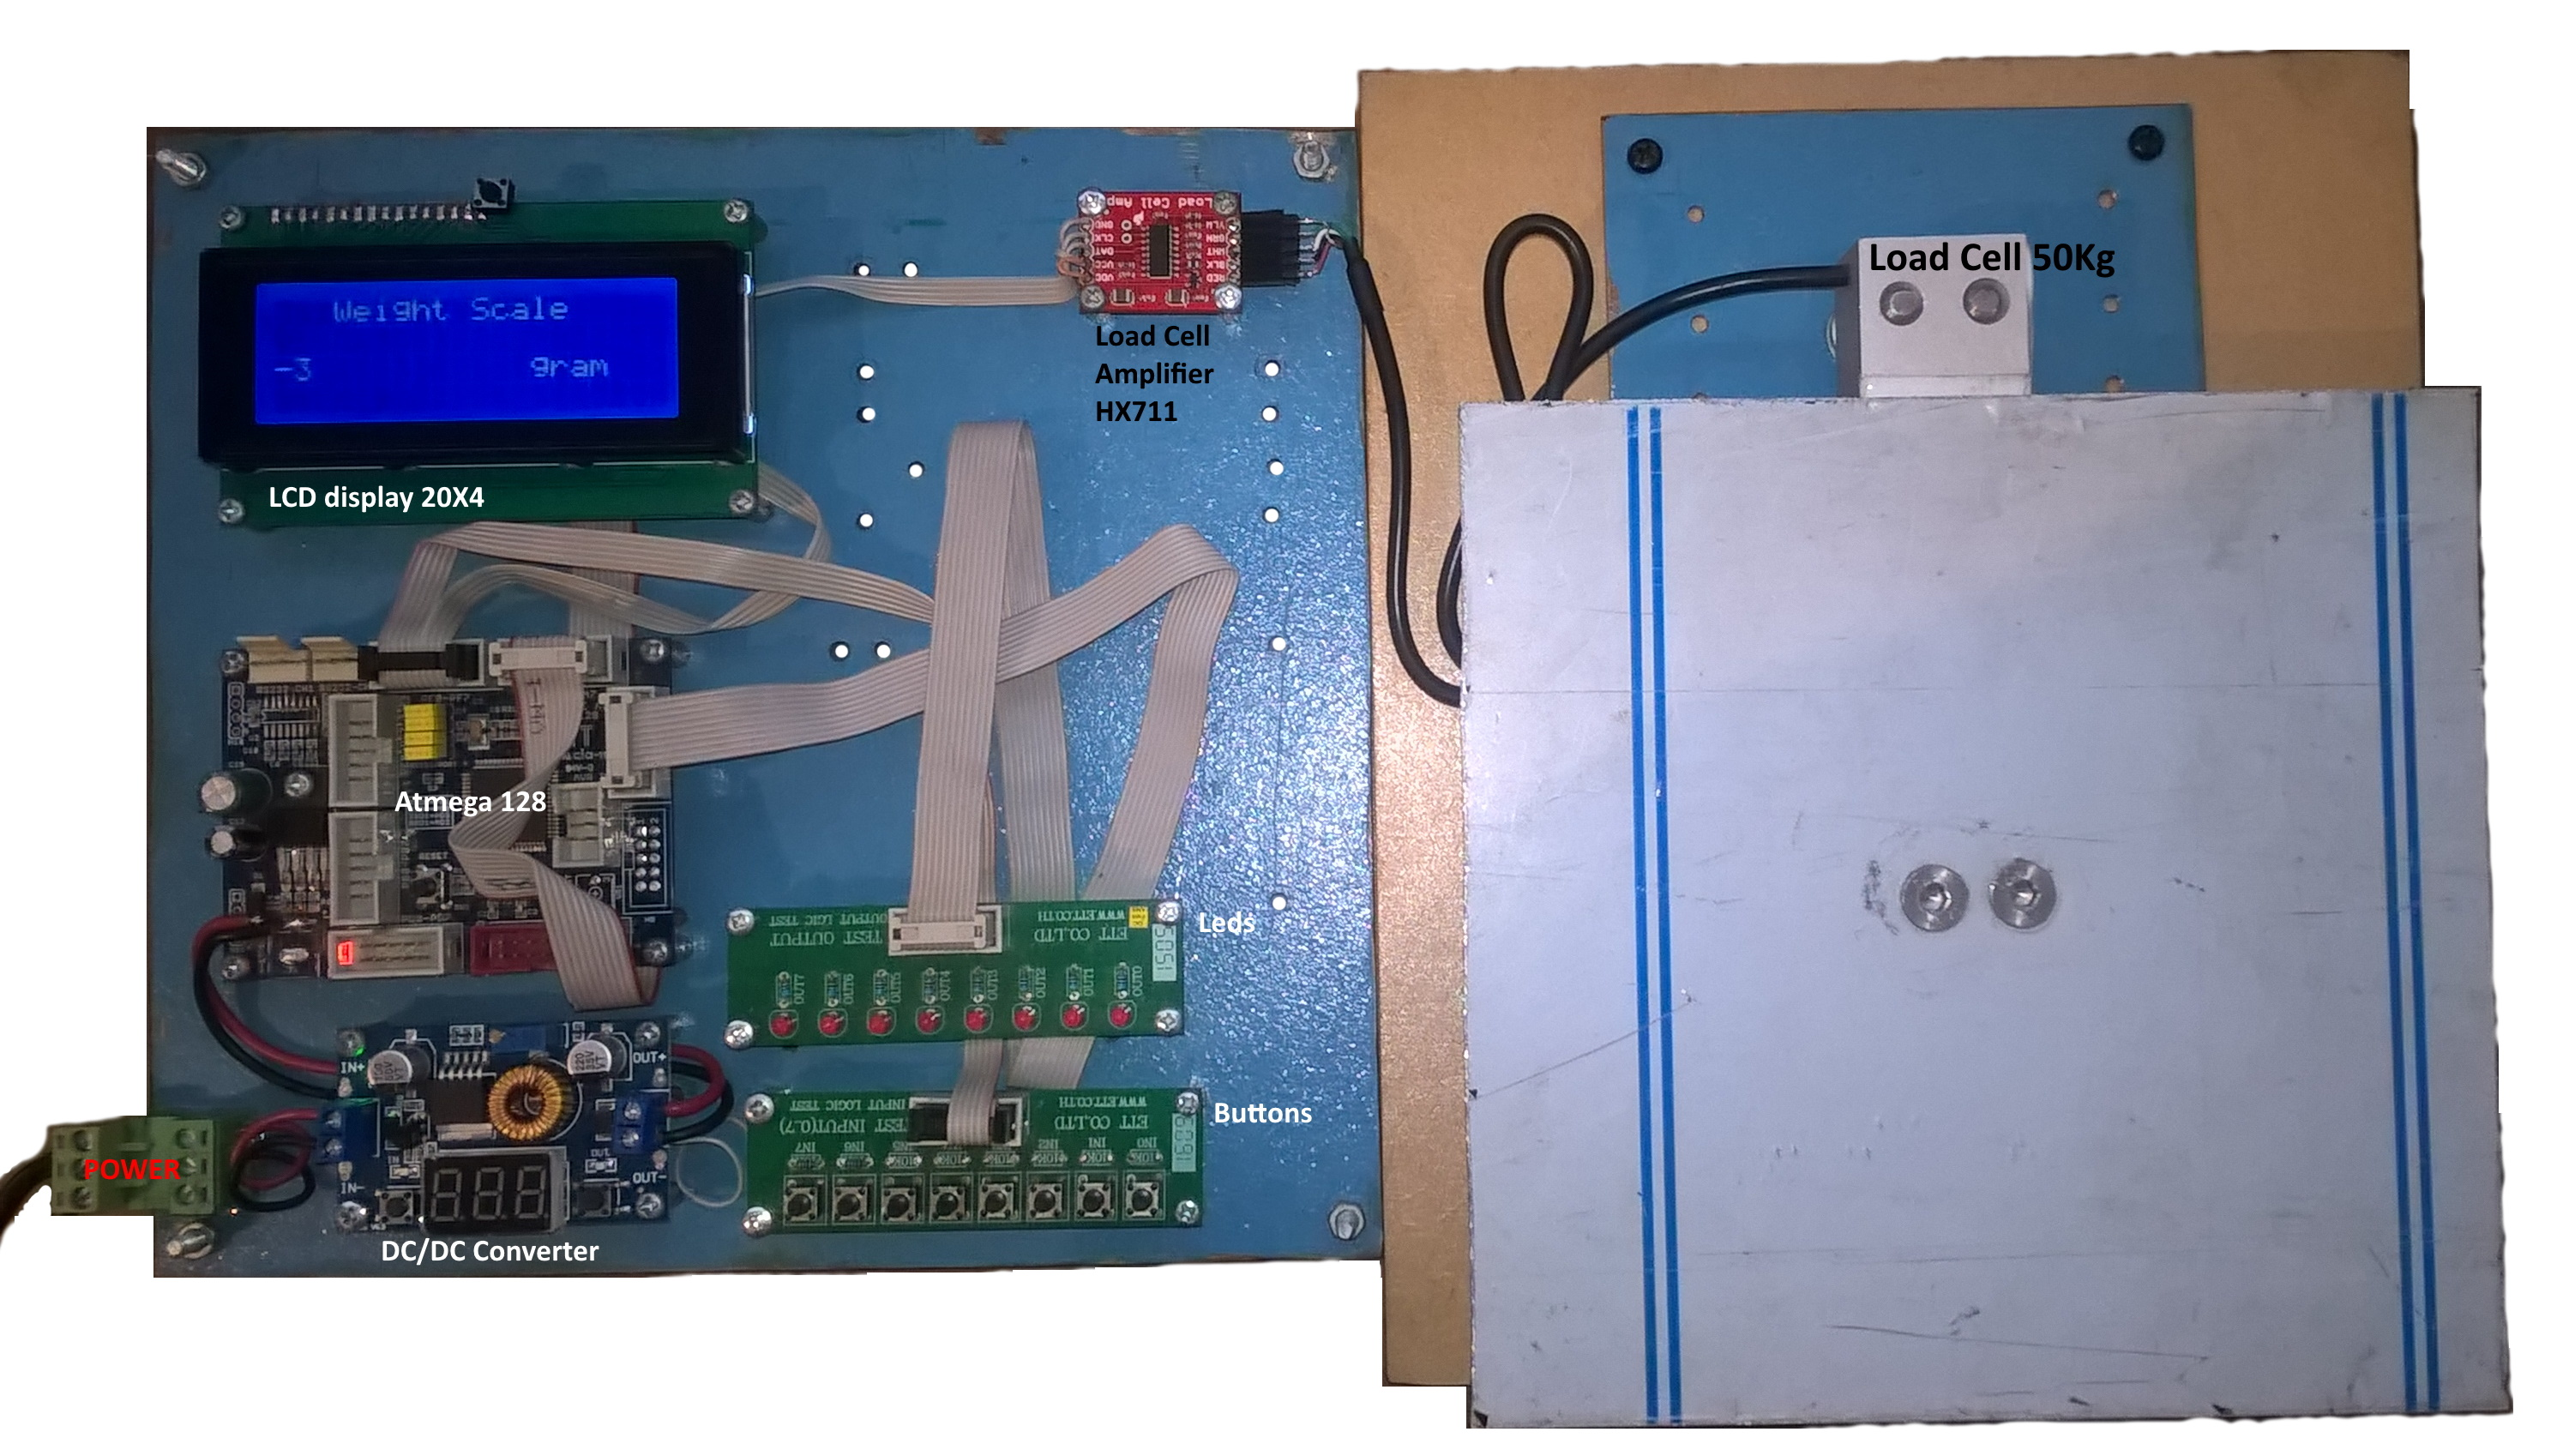
\includegraphics[scale=0.15]{./image/PESTA/kit/Kit_Desenvolvimento_2.jpg}
	\caption{Kit de Desenvolvimento}
	\label{Kit_Desenvolvimento_2}
\end{figure}
\newpage
A montagem da mesa de medição,
\begin{figure}[H]
	\centering
	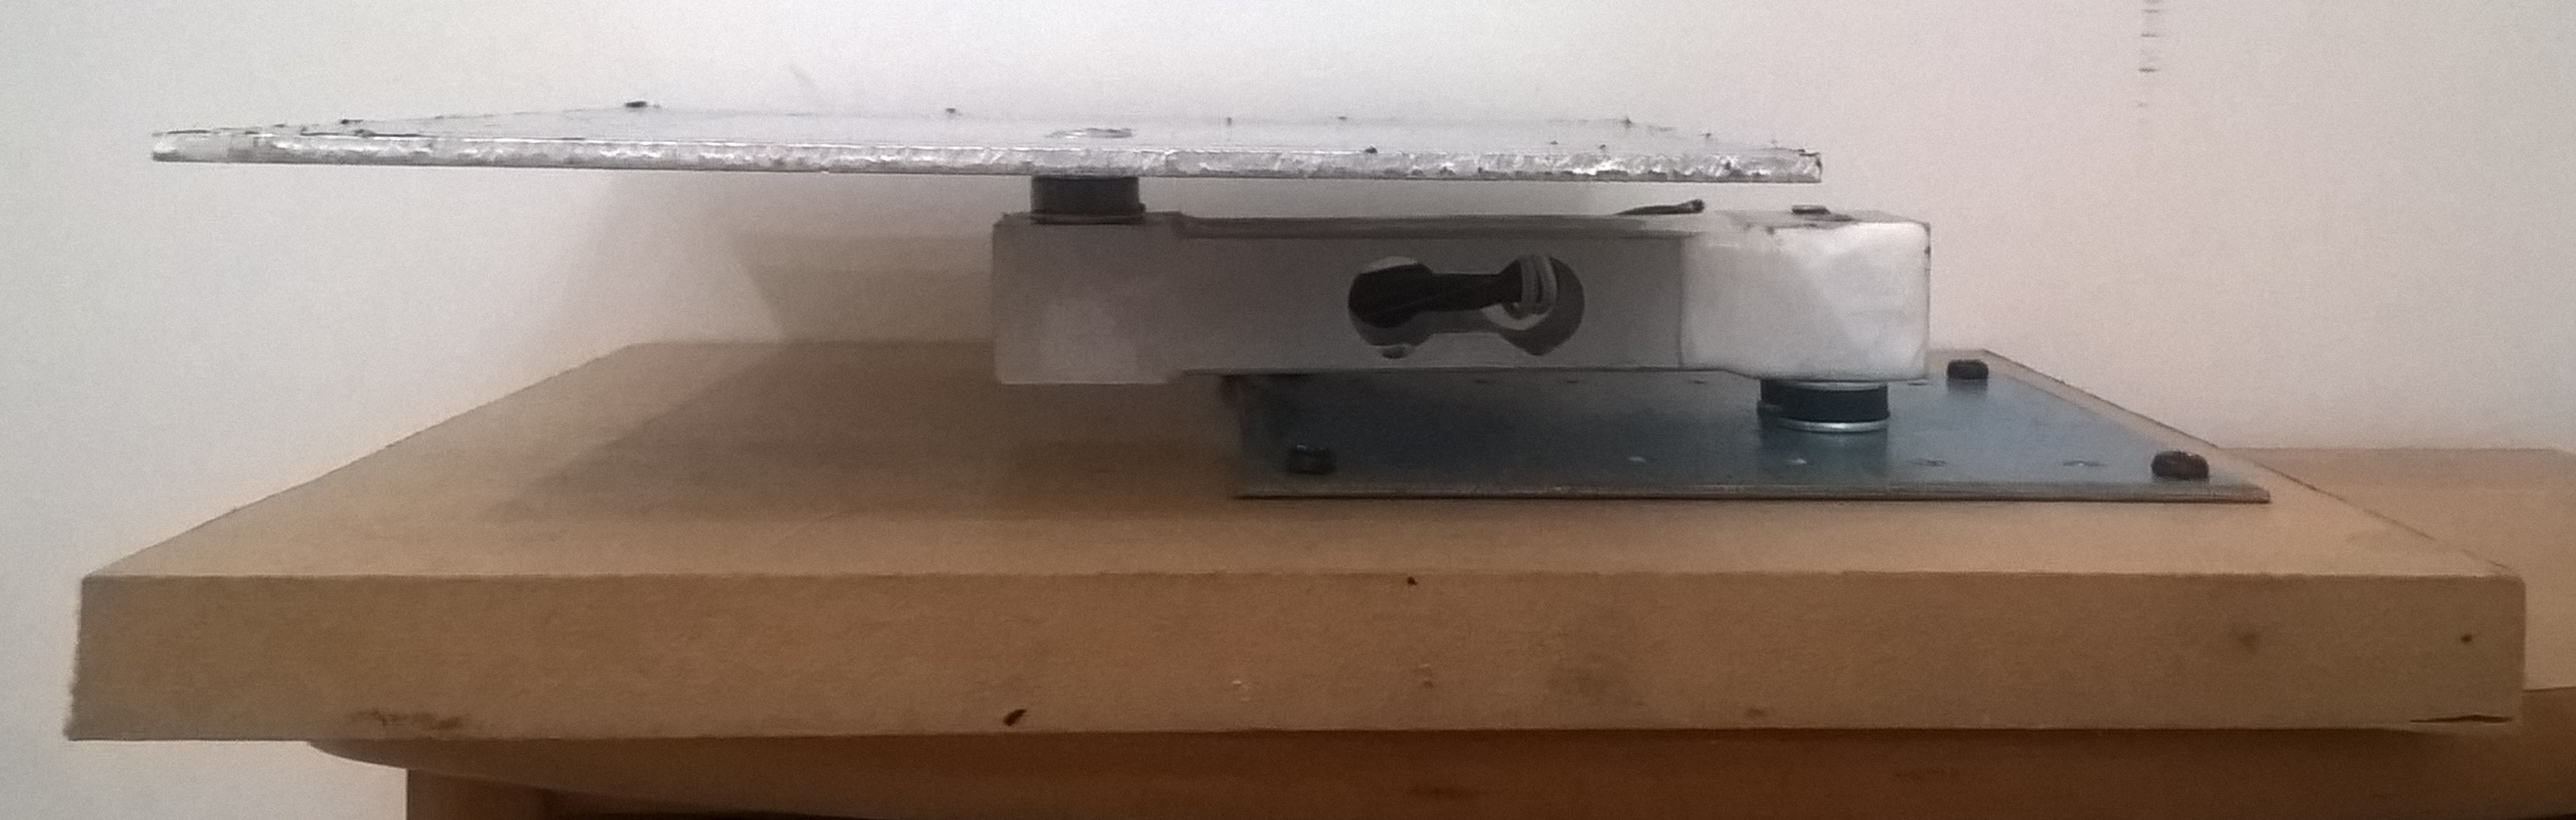
\includegraphics[scale=0.15]{./image/PESTA/material/Prato.jpg}
	\caption{Prato}
	\label{Prato}
\end{figure}
\subsection{Material}
Abaixo esta indicado uma tabela dos materiais usados, assim como os preços. 
\begin{table}[H]
	{\rowcolors{3}{blue!80!yellow!50}{blue!70!yellow!40}
		\begin{tabular}{ |p{12cm}|c|p{2cm}|  }
			\hline
			\multicolumn{3}{|c|}{Lista de Material} \\
			\hline
			Peça & Quant & Preço [uni] \\
			\hline
			Fonte de alimetação 12V 1A & 1 & \EUR{3.87} \\
			Conversor DC-DC com voltímetro & 1 & \EUR{7.75} \\
			ET BASE AVR Atmega128 Board & 1 & \EUR{23.92} \\
			Test Input Board  & 1 & \EUR{3.71} \\
			Test Output Board & 1 & \EUR{3.71} \\
			IDC Socket 10 way    & 12 & \EUR{0.31} \\
			IDC Header Straight 10 way    & 12 & \EUR{0.25} \\
			Flatcable    & ? & \EUR{?} \\
			20x4 LCD Module Blue & 1 & \EUR{12.24} \\
			SparkFun Load Cell Amplifier HX711 & 1 & \EUR{13.04}   \\
			50Kg Load Cell & 1 & \EUR{12} \\
			\hline
			 & \textit{total} & \EUR{86.96} \\
			\hline
		\end{tabular}
	}
	\caption{Lista de material}
	\label{material}
\end{table}
\newpage
\section{Funcionamento}
A ligação destes componentes é intuitivo e fácil de se perceber, o que é complexo neste trabalho é a interligação destes equipamentos com o micro-controlador e criar o driver de comunicação para a placa do amplificador de sinal, já que o protocolo é proprietário.
\begin{figure}[H]
	\captionsetup{justification=raggedright,singlelinecheck=false}
	\centering
	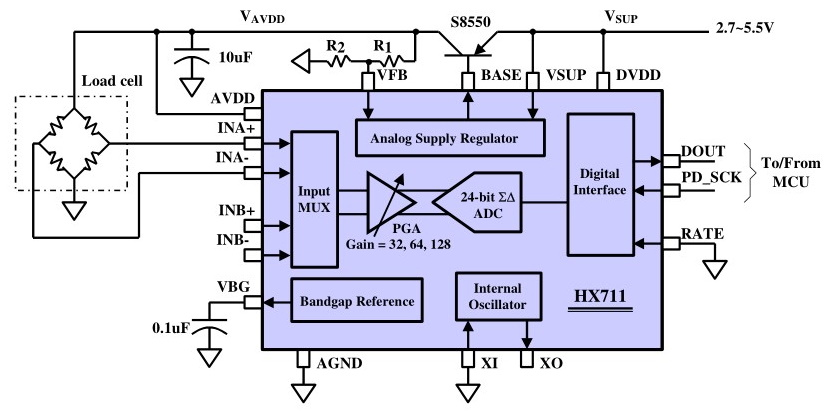
\includegraphics[scale=0.35]{./image/PESTA/schematic/HX711_Schematic_1.jpg}
	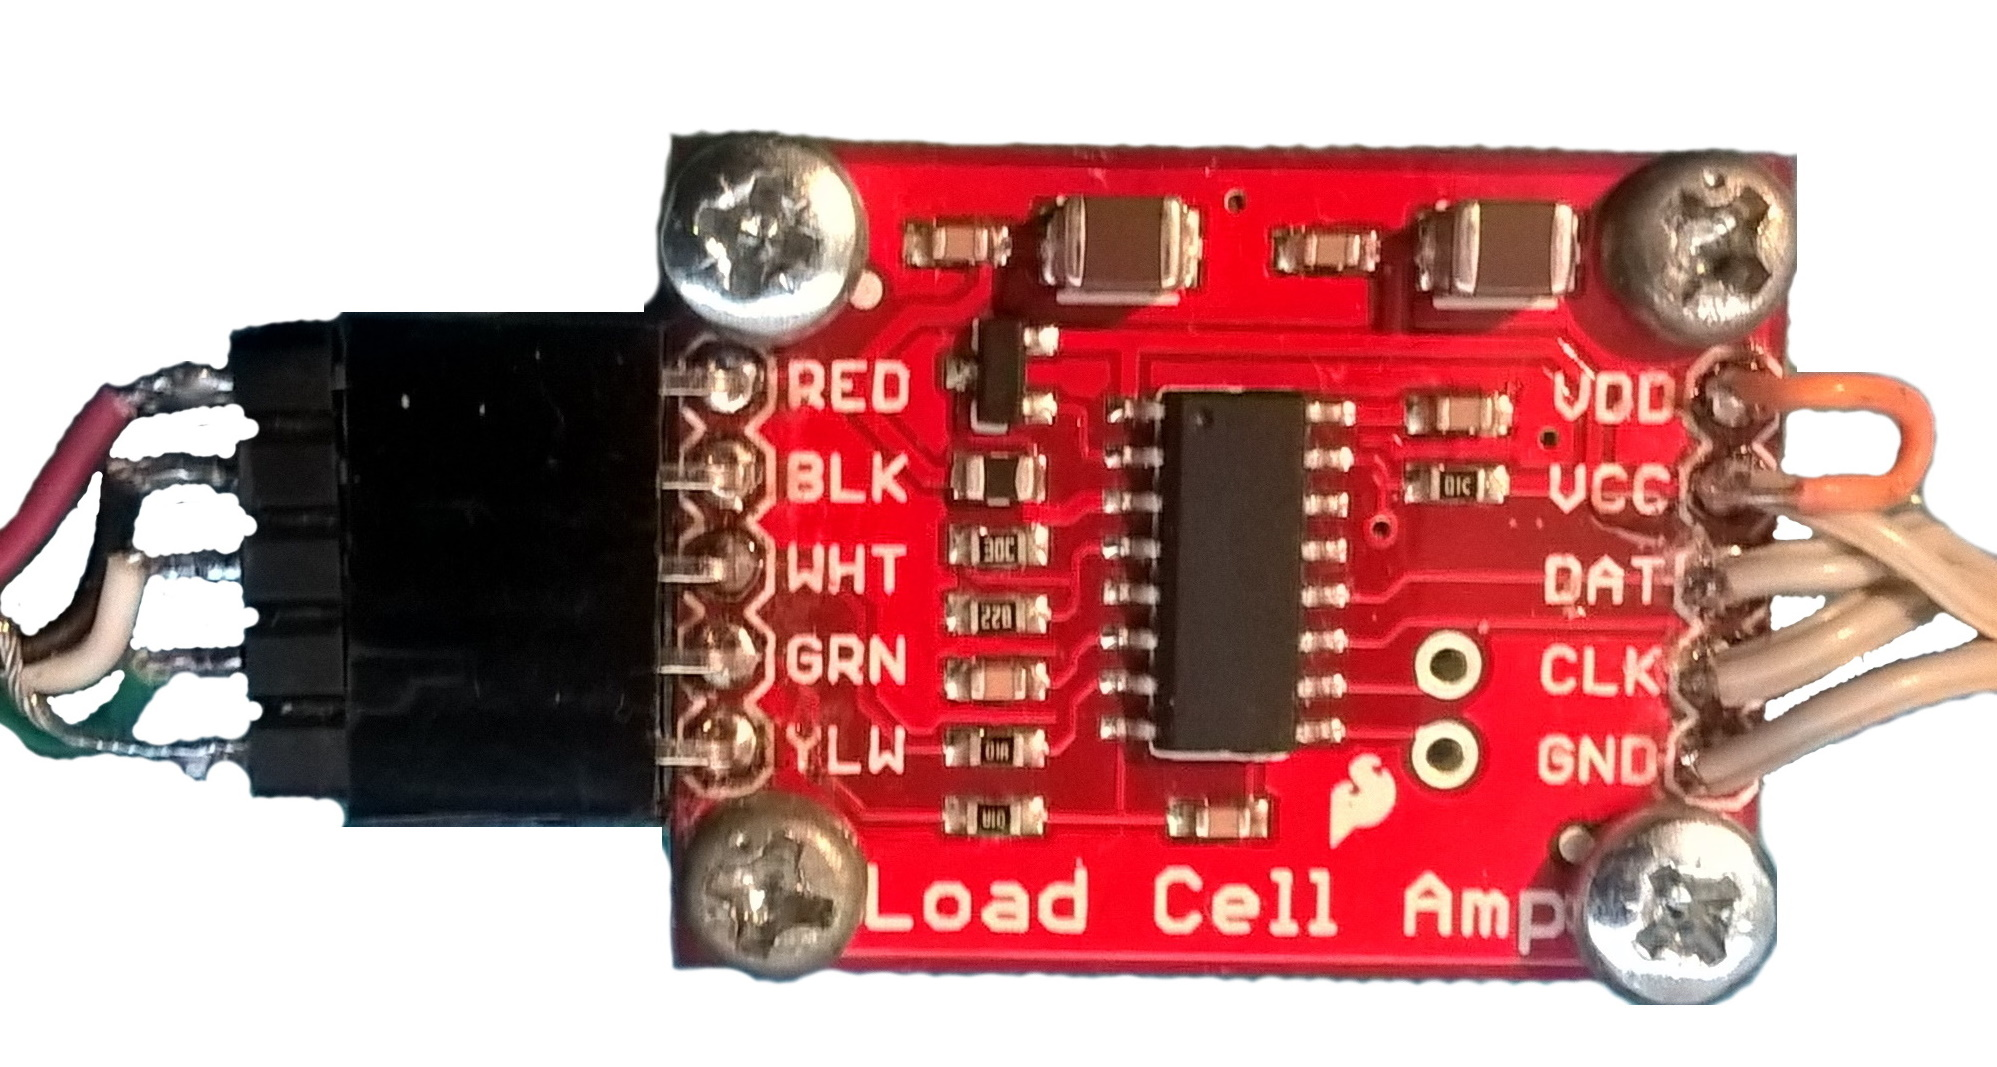
\includegraphics[scale=0.1]{./image/PESTA/material/HX711_board_1.jpg}
	\caption{Amplificador de Sinal [HX711]}
	\label{HX711_Schematic_1}
\end{figure}
A placa pode ser programada fisicamente para determinar o numero de amostras por segundo a ser transmitido, tem opção de \textcolor{blue}{10} amostras por segundo e \textcolor{blue}{80} amostras, neste projeto optei pela segunda opção que necessita alteração na placa de circuito de impresso, isto é, abrir o \textit{jumper} respetivo de configuração.
\begin{figure}[H]
	\centering
	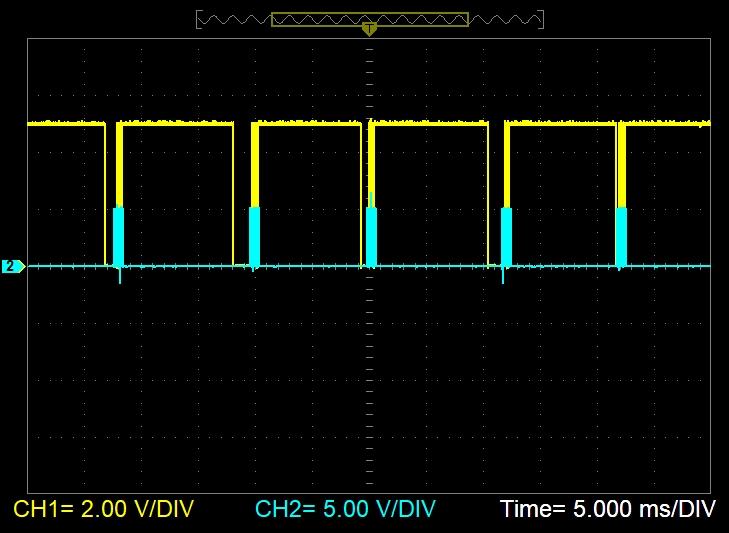
\includegraphics[scale=0.55]{./image/PESTA/graph/80SPS64GAIN/SPS_80.JPG}
	\caption{Amostras}
	\label{SPS_64}
\end{figure}
A livraria (driver) recorre a interrupções quando o sinal de \textit{data} vai para a massa, indicando assim que tem um pacote de leitura pronto a ser transmitido.\\
\\
%%\begin{minipage}{\linewidth}
\begin{minipage}[!b]{.40\linewidth}
	\begin{table}[H]
		\captionsetup{justification=raggedright,singlelinecheck=false}
		\begin{tabular}{ | c | c | c |  }
			\hline
			\makecell[c]{PD\_SCK \\ Impulsos} & Entrada  & Ganho \\
			\hline
			\hline
			25 & \textbf{A} & 128 \\
			\hline
			26 & \textbf{B} & 32 \\
			\hline
			27 & \textbf{A} & 64 \\
			\hline
		\end{tabular}	
		\caption{Configuração Ganho}
		\label{Gain_Selection}
	\end{table}
	\vfill
\end{minipage}
\begin{minipage}[l]{.6\linewidth}
\vspace{.3cm}
Como indicado abaixo no gráfico em que a linha amarela é a informação e a linha azul o respetivo \textit{clock} que é gerado pelas interrupções do micro-controlador fazendo \textit{shift} dos \textcolor{blue}{24} bits, que depois no fim transmite para o amplificador o ganho de amplificação a ser usado pelo numero excedente de \textit{clock cycles}, que nesta demonstração é \textcolor{blue}{um}, e corresponde a ganho de \textcolor{blue}{128}, respeitando a \textit{tabela} \ref{Gain_Selection}.
\end{minipage}\\
\\
%%\end{minipage}
\begin{figure}[H]
	\centering
	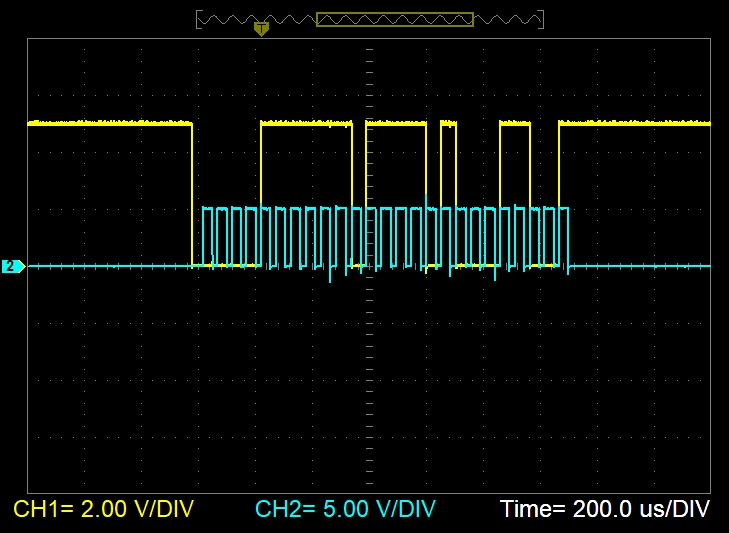
\includegraphics[scale=0.35]{./image/PESTA/graph/80SPS128GAIN/Gain_128_example.JPG}
	\caption{Ganho de 128}
	\label{Gain_128_example}
\end{figure}
a sequir o exemplo com o ganho de \textcolor{blue}{64}, pois tem \textcolor{blue}{três} impulsos excedentes.
\begin{figure}[H]
	\centering
	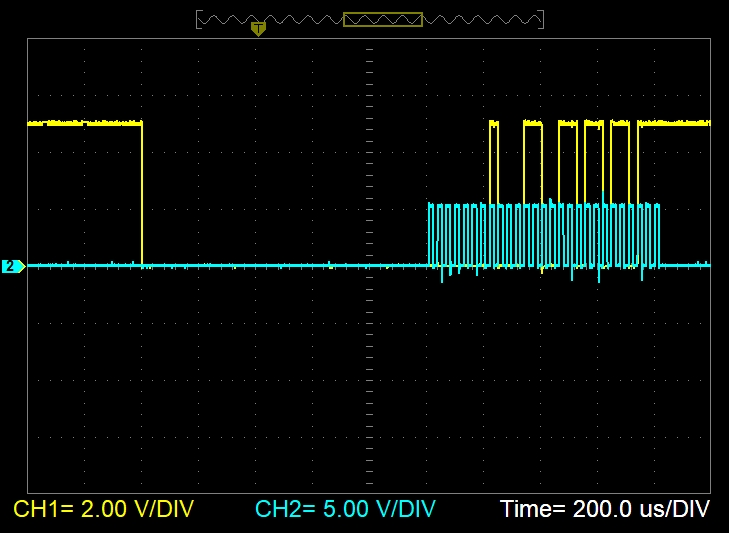
\includegraphics[scale=0.35]{./image/PESTA/graph/80SPS64GAIN/Gain_64_example.JPG}
	\caption{Ganho de 64}
	\label{Gain_64_example}
\end{figure}
Para obter este resultado uma livraria driver para o \textit{Load Cell Amplifier} foi criado tendo em consideração que o microcontrolador é de \textcolor{blue}{8} bits. O pacote de informação consiste de \textcolor{blue}{24} bits na qual é transmitido primeiro o bit \textbf{MSB}.
\newpage
O codigo que executa esta rotina é demonstrado.
\begin{figure}[H]
	\centering
	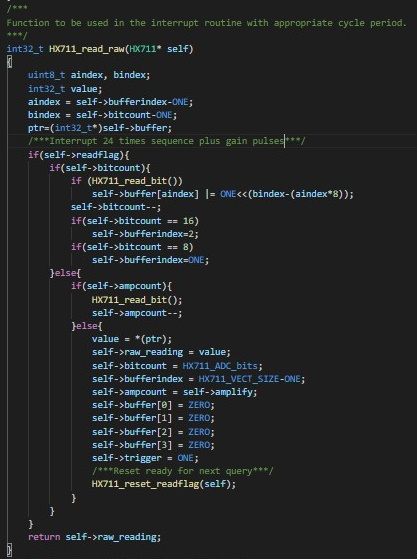
\includegraphics[scale=0.8]{./image/PESTA/Code/read_raw.jpg}
	\caption{Leitura ADC}
	\label{read_raw}
\end{figure}
após obter um numero determinado de valores discretos é calculado sua média $\left( \overline{x}  =  \frac{1}{n}\sum_{i=1}^n x_i \right)$ para ser tratado e deduzido o valor correspondente de sua massa. \\
\\
Uma analise rápida do código também é possível de se perceber o funcionamento da livraria do driver que será anexado a este relatório e disponível no \textit{link}: \url{https://github.com/sergio1020881/PESTA2021/tree/main/SandBox/ATMEGA128/Atmega128}
\newpage
\section{Software}
software, flowchart, programming equipament.


\newpage
\section{Validação}
%%%To validate is to justify why the choices made and alternatives that could be chosen.
As escolhas feitas estão dentro dos parâmetros na qual a oferta nos disponibiliza, sendo que pouco se pode beneficiar. Apenas o conhecimento adquirido e aprofundar o funcionamento é o ganho mais evidente, facilitando a interpretação de situações e deteção de anomalias (\textit{troubleshooting}).\\
\\
Apostei na marca \textbf{Atmel} devido a experiência adquirida, conjunto de já conhecimentos adquiridos e de me ser familiar, sendo que se aposta-se noutra marca teria de enfrentar uma curva de aprendizagem e adaptação que no final a nível de custos beneficio seria desfavorável, muito trabalhoso.\\
\\
O sensor usado é o mais comum nesta pratica, e escolha demonstrada, o circuito de interface é indiferente a escolha apenas é baseada na sua precisão, ou seja, é de \textcolor{blue}{24} \textit{bit}, e o \textit{chip} apenas tem  de \textcolor{blue}{10} \textit{bit} de resolução.





%%%%%%%%%%%%%%%%%%%%%%%%%%%%%%%%%%%%%%%%%%%%%%%%%%%%%%%%%%%%%%%%
\begin{comment}
Sem contar com as despesas no equipamento para a programação do hardware que em principio só se gasta uma vez, isto é, se não se estragar. No caso do programador \textbf{Atmel-ICE} pode custar até \EUR{185.55}.\\
\\
É de ter em conta que os preços são \textbf{PVP}, que no caso se for preços comerciais são dez vezes inferior, e se for para produção em grande escala também tem descontos por quantidade.\\
$\begin{array}{l l l}
\text{Média} & & \\
\overline{x} & = & \frac{1}{n}\sum_{i=1}^n x_i
\end{array}$
MEMS devices and structures are fabricated using conventional integrated circuit
process techniques, such as lithography, deposition, and etching, together with a
broad range of specially developed micromachining techniques. \cite{book-9}
The three essential elements in conventional
silicon processing are deposition, lithography, and etching. \cite{book-9}
Sensitivity,Long-Term Drift e Temperature Effects (Span temperature hysteresis).
\end{comment}
%%%%%%%%%%%%%%%%%%%%%%%%%%%%%%%%%%%%%%%%%%%%%%%%%%%%%%%%%%%%%%%%